\chapter{Matrix-Matrix Product}

The matrix-matrix product is a binary operation that produces 
another matrix from two matrices. For the procedure to be valid, 
the number of columns of the first matrix must be equal to the 
rows of the second matrix. The resulting matrix's dimension is 
an amalgam of the dimension of the two matrics.

Let the first matrix be $A$ with the dimensions $m \times k$; 
the second matrix be $B$ with the dimensions $n \times k$, 
and the result matrix be $C$.

Hence, the dimensions of the matrix $C$ will be $m \times n$.

\[
A= 
\begin{bmatrix}
    a_{00}  & a_{01}    & \dots     & a_{0k}\\
    a_{10}  & a_{11}    & \dots     & a_{1k}\\
    \vdots  & \vdots    & \ddots    & \vdots\\
    a_{m0}  & a_{m1}    & \dots     & a_{mk}\\
\end{bmatrix}
,
B= 
\begin{bmatrix}
    b_{00}  & b_{01}    & \dots     & b_{0n}\\
    b_{10}  & b_{11}    & \dots     & b_{1n}\\
    \vdots  & \vdots    & \ddots    & \vdots\\
    b_{k0}  & b_{k1}    & \dots     & b_{kn}\\
\end{bmatrix}
,
C= 
\begin{bmatrix}
    c_{00}  & c_{01}    & \dots     & c_{0n}\\
    c_{10}  & c_{11}    & \dots     & c_{1n}\\
    \vdots  & \vdots    & \ddots    & \vdots\\
    c_{m0}  & c_{m1}    & \dots     & c_{mn}\\
\end{bmatrix}
\]

\vspace*{0.5cm}

\begin{equation}
    C = A \times B
\end{equation}

\[
\begin{bmatrix}
    c_{00}  & c_{01}    & \dots     & c_{0n}\\
    c_{10}  & c_{11}    & \dots     & c_{1n}\\
    \vdots  & \vdots    & \ddots    & \vdots\\
    c_{m0}  & c_{m1}    & \dots     & c_{mn}\\
\end{bmatrix}
= 
\begin{bmatrix}
    a_{00}  & a_{01}    & \dots     & a_{0k}\\
    a_{10}  & a_{11}    & \dots     & a_{1k}\\
    \vdots  & \vdots    & \ddots    & \vdots\\
    a_{m0}  & a_{m1}    & \dots     & a_{mk}\\
\end{bmatrix}
\times
\begin{bmatrix}
    b_{00}  & b_{01}    & \dots     & b_{0n}\\
    b_{10}  & b_{11}    & \dots     & b_{1n}\\
    \vdots  & \vdots    & \ddots    & \vdots\\
    b_{k0}  & b_{k1}    & \dots     & b_{kn}\\
\end{bmatrix}
\]

\vspace*{0.5cm}

\begin{equation}
    c_{i,j} = \sum_{l=0}^k (a_{i,l} \times b_{l,j})
\end{equation}

\clearpage

\section{Algorithm}

The algorithm we implemented using OpenMP came from the \cite{BLIS}, 
and we simply following the algorithm provided in the paper 
and all the tuning parameter also comes from the same paper using 
their calculation. However, there are a few difference in the 
calculation because we cannot control the assembly which emitted 
by the compiler. The calculation is not far from the initially 
provided by the paper.

\begin{algorithm}[H]
    \SetAlgoLined
    \SetKwFunction{SIMDFn}{$simd\_loop$}
    \SetKwProg{Fn}{Function}{:}{end}

    \tcp{$c$    is the pointer to the output Matrix}
    \tcp{$ldc$  is leading dimension of the output Matrix}
    \tcp{$a$    is the pointer to the input Matrix}
    \tcp{$b$    is the pointer to the input Matrix}
    \tcp{$k_c$  is the block of the Matrix in the contracting dimension}
    \tcp{$m$    is the block of the Matrix $A$ in the non-contracting dimension}
    \tcp{$n$    is the block of the Matrix $B$ in the non-contracting dimension}
    \tcp{$M_r$  is the micro-tile of the Matrix $A$ in the non-contracting dimension}
    \tcp{$N_r$  is the micro-tile of the Matrix $B$ in the non-contracting dimension}
    \Fn{\SIMDFn($c$, $ldc$, $a$, $b$, $k_c$, $m$, $n$)}{
        \assignln{buff_{M_r \times N_r}}{0}
        \assignln{half_{N_r}}{\frac{N_r}{2}}
        \For{\assign{k}{0} \KwTo $k_c$ \KwBy $1$}{
            \For{\assign{j}{0} \KwTo $half_{N_r}$ \KwBy $1$}{
                \openmp{simd}
                \For{\assign{i}{0} \KwTo $M_r$ \KwBy $1$}{
                    \assignln{buff[j \times M_r + i]}{buff[j \times M_r + i] + bk[j] \times ak[i]}
                    \assignln{buff[(j + half_{N_r}) \times M_r + i]}{buff[j \times M_r + i] + bk[j + half_{N_r}] \times ak[i]}
                }
            }
        }
        \tcp{Copy the $buff$ into the output Matrix $c$}
    }
    \caption{Matrix-Matrix Product SIMD Function}
\end{algorithm}

\begin{algorithm}[H]
    \SetAlgoLined
    \SetKwFunction{MicroKernel}{$micro\_kernel$}
    \SetKwProg{Fn}{Function}{:}{end}

    \tcp{$c$    is the pointer to the output Matrix}
    \tcp{$w_c$  is pointer to the strides of the output Matrix}
    \tcp{$a$    is the pointer to the input Matrix}
    \tcp{$w_a$  is pointer to the strides of the output Matrix}
    \tcp{$b$    is the pointer to the input Matrix}
    \tcp{$w_b$  is pointer to the strides of the output Matrix}
    \tcp{$M$    is the block of the Matrix $A$ in the non-contracting dimension}
    \tcp{$N$    is the block of the Matrix $B$ in the non-contracting dimension}
    \tcp{$K$    is the block of the Matrix in the contracting dimension}
    \tcp{$M_r$  is the micro-tile of the Matrix $A$ in the non-contracting dimension}
    \tcp{$N_r$  is the micro-tile of the Matrix $B$ in the non-contracting dimension}
    \Fn{\MicroKernel($c$, $ldc$, $a$, $b$, $M$, $N$, $K$)}{
        \assignln{ldc}{max(w_c[0],w_c[1])}

        \For{\assign{j}{0} \KwTo $N$ \KwBy $N_r$}{
            \assignln{a_i}{a}
            \assignln{b_i}{b + j \times K}
            \assignln{c_i}{c + j \times w_c[1]}
            \assignln{j_b}{max(N_r, N - j)}
            \For{\assign{i}{0} \KwTo $M$ \KwBy $M_r$}{
                \assignln{a_k}{ai + i \times K}
                \assignln{b_k}{bi}
                \assignln{c_k}{ci + i \times w_c[o]}
                \assignln{i_b}{max(M_r, M - i)}
                $simd\_loop(c_k, ldc, a_k, b_k, K, i_b, j_b)$
            }
        }
    }
    \caption{Matrix-Matrix Product Micro-Kernel}
\end{algorithm}

\begin{algorithm}[H]
    \SetAlgoLined
    \KwIn{$c$, $n_c$, $w_c$ $a$, $n_a$, $w_a$, $b$, $n_b$, $w_b$, $max\_threads$}
    \tcp{$c$    is the pointer to the output Matrix}
    \tcp{$n_c$  is pointer to the dimensions of the output Matrix}
    \tcp{$w_c$  is pointer to the strides of the output Matrix}
    \tcp{$a$    is the pointer to the input Matrix}
    \tcp{$n_a$  is pointer to the dimensions of the output Matrix}
    \tcp{$w_a$  is pointer to the strides of the output Matrix}
    \tcp{$b$    is the pointer to the input Matrix}
    \tcp{$n_b$  is pointer to the dimensions of the output Matrix}
    \tcp{$w_b$  is pointer to the strides of the output Matrix}
    \tcp{$max\_threads$ is the user provided thread count}
    \tcp{$M_B$   is the block of the Matrix $A$ in the non-contracting dimension}
    \tcp{$N_B$   is the block of the Matrix $B$ in the non-contracting dimension}
    \tcp{$K_B$   is the block of the Matrix in the contracting dimension}
    \tcp{$M_r$  is the micro-tile of the Matrix $A$ in the non-contracting dimension}
    \tcp{$N_r$  is the micro-tile of the Matrix $B$ in the non-contracting dimension}

    \Begin{

        \assignln{M}{na[0]}
        \assignln{N}{nb[1]}
        \assignln{K}{nb[0]}

        \assignln{a_i}{a}
        \assignln{b_i}{b}
        \assignln{c_i}{c}
        
        \assignln{buff\_size_A}{K_B \times ( M_B + 1 ) \times max\_threads}
        \assignln{buff\_size_B}{K_B \times ( N_B + 1 )}

        $buff_A(buff\_size_A)$
        
        $buff_B(buff\_size_B)$
        
        \openmp{parallel}
        \Begin{
            \For{\assign{j}{0} \KwTo $N$ \KwBy $N_B$}{
                \assignln{a_k}{a_i}
                \assignln{b_k}{b_i + j \times w_b[1]}
                \assignln{c_k}{c_i + j \times w_c[1]}
                \assignln{j_b}{max(N_B, N - j)}
                \For{\assign{k}{0} \KwTo $K$ \KwBy $K_B$}{
                    \assignln{a_i}{a_k + k \times w_a[1]}
                    \assignln{b_i}{b_k + k \times w_b[0]}
                    \assignln{c_i}{c_k}
                    \assignln{k_b}{max(K_B, K - j)}
                    \tcp{Pack $B$ into $buff_B$}

                    \openmp{for schedule(dynamic)}
                    \For{\assign{i}{0} \KwTo $M$ \KwBy $M_B$}{
                        \assignln{t_{id}}{omp\_get\_thread\_num()}
                        \assignln{a_j}{a_j + i \times w_a[0]}
                        \assignln{b_j}{b_j}
                        \assignln{c_j}{c_j + i \times w_c[0]}
                        \assignln{i_b}{max(M_B, M - i)}
                        \tcp{Pack $A$ into $buff_A$}
                        $micro\_kernel(c_j, w_c, (buff_A + t_{id} \times k_b \times M_B), buff_B, i_b, j_b, k_b)$
                    }
                }
            }
        }

    }

    \caption{Matrix-Matrix Product}
\end{algorithm}

\section{Tuning Parameter}

If the reader wants to know the reasoning and rationale 
behind each of the derivation of the tuning parameter, 
they may read the original \cite{BLIS} paper.

\subsection{Micro-Tiles $M_r$ and $N_r$}
\label{sec:mr_nr_calculation}

Let $L_{VFMA}$ and $N_{VFMA}$ be the latency and throughput of the FMA instruction, 
$N_{VEC}$ be the width of the vector register, and
$L_{L/S}$ and $N_{L/S}$ be the latency and throughput of 
the Load and Store instruction.

Using equation from the \cite{BLIS}, we get

\begin{equation}
    M_rN_r \geq N_{VEC} L_{effective} N_{effective}
\end{equation}

To find the effective latency and throughput, we cannot directly take the 
algebraic sum for the throughput, which will give the wrong result. Instead, taking the 
algebraic sum of the latency gives the actual effective latency, 
and taking the harmonic mean gives the effective throughput.

\begin{align*}
    L_{effective} &= 2L_{L/S} + L_{VFMA}\\
    N_{effective} &= \frac{3}{ \frac{1}{N_{VEC}} + \frac{1}{2N_{L/S}} } \\
\end{align*}

\begin{align*}
    M_r &= \lceil \frac{ \sqrt{N_{VEC} L_{effective} N_{effective}} }{N_{VEC}} \rceil N_{VEC} \\
    N_r &= \lceil \frac{ N_{VEC} L_{effective} N_{effective} }{M_r} \rceil
\end{align*}


Calculating $M_r$ and $N_r$ for Intel SkyLake with the AVX2.

\begin{table}[ht]
    \centering
    \caption{Latency and Throughput}
    \begin{tabular}{|l|c|c|}
        \hline
        \textbf{Instruction} & \textbf{Latency} & \textbf{Throughput}\\
        \hline
        VFMA        & $4$ & $0.5$ \\
        \hline
        Load/Store  & $7$ & $0.5$ \\
        \hline
    \end{tabular}
\end{table}

$N_{VEC} = 8$ for Single-Precision and $N_{VEC} = 4$ for Double-Precision.

\begin{align*}
    M_r &= \lceil \frac{ \sqrt{9 N_{VEC}} }{N_{VEC}} \rceil N_{VEC} \\
    N_r &= \lceil \frac{ 9 N_{VEC} }{M_r} \rceil
\end{align*}

\begin{table}[ht]
    \centering
    \caption{Tuning Parameter $M_r$ and $N_r$ for Intel SkyLake with the AVX2}
    \begin{tabular}{|c|c|c|}
        \hline
        \textbf{Tuning Parameter} & \textbf{Single} & \textbf{Double}\\
        \hline
        $M_r$   & $16$ & $8$ \\
        \hline
        $N_r$   & $6$ & $6$ \\
        \hline
    \end{tabular}
\end{table}

\subsection{Macro-Tiles $M_B$, $N_B$ and $K_B$}

Let $C_{A_r}$ and $C_{B_r}$ be the number of cache line taken by the micro-tile $A_r$ and $B_r$.

Similarly, to derive the $K_B$, we will use the derivation from the \cite{BLIS}, which is 
mapped to the parameter $k_c$ in the paper.

According to the paper, if we do not want the micro-tile of $B_r$ 
to replaced by the new micro-tile of $A_r$, the $C_{A_r}$ and $C_{B_r}$  should 
follow the below constraint.

\[C_{A_r} + C_{B_r} \leq W_{L_1}\]

But here, we also need to consider the cache line of the micro-tile of $C$, which will $L_1$
cache as the route to the register.

\begin{equation}
    C_{A_r} + C_{B_r} \leq W_{L_1} - 1
    \label{eq:mtm_tuning_CAr_CBr}
\end{equation}

We know that

\begin{equation}
    M_r K_B S_{data} = C_{A_r} N_{L_1} C_{L_1}
    \label{eq:mtm_tuning_KB_CAr}
\end{equation}

\begin{equation}
    N_r K_B S_{data} = C_{B_r} N_{L_1} C_{L_1}
    \label{eq:mtm_tuning_KB_CBr}
\end{equation}

Dividing the \ref{eq:mtm_tuning_KB_CAr} and \ref{eq:mtm_tuning_KB_CBr}, we get

\begin{align*}
    \frac{C_{A_r}}{C_{B_r}} = \frac{M_r}{N_r}
\end{align*}

Here we part ways little bit from the paper and we take floor rather than ceil.

\begin{equation}
    C_{B_r} = \lfloor \frac{N_r}{M_r} C_{A_r} \rfloor
    \label{eq:mtm_tuning_CBr}
\end{equation}

Substituting the \ref{eq:mtm_tuning_CBr} into the \ref{eq:mtm_tuning_CAr_CBr}, we get
\begin{align*}
    &C_{A_r} \lfloor ( 1 + \frac{N_r}{M_r} ) \rfloor = W_{L_1} - 1\\
    &C_{A_r} = \lceil \frac{W_{L_1} - 1}{1 + \frac{N_r}{M_r}} \rceil\\
\end{align*}

\begin{table}[ht]
    \centering
    \caption{Cache Info for the Intel SkyLake}
    \begin{tabular}{|c|c|c|c|}
        \hline
        \textbf{Level} & \textbf{$W_{L_i}$} & \textbf{$N_{L_i}$} & \textbf{$C_{L_i}$}\\
        \hline
        $L_1$   & $8$ & $64$ & $64$ \\
        \hline
        $L_2$   & $4$ & $1024$ & $64$ \\
        \hline
        $L_3$   & $16$ & $16Ki$ & $64$ \\
        \hline
    \end{tabular}
\end{table}

\[
    C_{A_r} = \lceil \frac{7}{1 + \frac{N_r}{M_r}} \rceil
\]

Substituting the $C_{A_r}$ into the equation \ref{eq:mtm_tuning_KB_CAr}.

\begin{table}[ht]
    \centering
    \caption{Tuning Parameter $K_B$}
    \begin{tabular}{|c|c|c|}
        \hline
        \textbf{Tuning Parameter} & \textbf{Single} & \textbf{Double}\\
        \hline
        $K_B$   & $384$ & $256$ \\
        \hline
    \end{tabular}
\end{table}

To get $M_B$, we do the same process as we did to find $K_B$, but we need to fill 
the macro-block of matrix $A$ into the $L_2$ cache.

\[C_{A_c} + C_{B_r} \leq W_{L_2} - 1\]
\[C_{A_c} = W_{L_2} - 1 - C_{B_r}\]

We the $C_{B_r}$ from the equation \ref{eq:mtm_tuning_CBr}. Here, there is a catch what if
the $C_{A_c}$ comes out to be $0$. Therefore, to avoid the this problem can derive the 
relationship between the $C_{A_c}$ and $C_{B_r}$.

\begin{align*}
    M_B K_B S_{data} &= C_{A_c} N_{L_2} C_{L_2}\\
    N_r K_B S_{data} &= C_{B_r} N_{L_2} C_{L_2}\\
\end{align*}

Now, dividing the both equation and we get

\begin{align*}
    \frac{C_{A_c}}{C_{B_r}} = \frac{M_B}{N_r}
\end{align*}

\begin{align*}
    &C_{A_c} \lfloor ( 1 + \frac{N_r}{M_B} ) \rfloor = W_{L_2} - 1\\
    &C_{A_c} = \lceil \frac{W_{L_2} - 1}{1 + \frac{N_r}{M_B}} \rceil\\
\end{align*}

Using the observation, we can see $M_B$ will be very large compared to the $N_r$. Therefore,
we reach to the conclusion that $N_r$ cannot be larger than the $M_B$ and can never be zero.
But their may be the case where they are same.


\begin{align*}
    0 &< \frac{N_r}{M_B} \leq 1\\
    1 &< 1 + \frac{N_r}{M_B} \leq 2\\
    \frac{1}{2} &\leq \frac{1}{1 + \frac{N_r}{M_B}} < 1\\
    \frac{W_{L_2} - 1}{2} &\leq \frac{W_{L_2} - 1}{1 + \frac{N_r}{M_B}} < W_{L_2} - 1\\
\end{align*}

For the best possible solution or performance, we chose the lower bound from the above equation.

\[
    C_{A_c} = \lfloor \frac{W_{L_2} - 1}{2} \rfloor
\]
\[
    M_B = \lfloor \frac{(W_{L_2} - 1)}{2} \rfloor \frac{N_{L_2} C_{L_2}}{K_B S_{data}}\\
\]

To the get the best optimal value of $M_B$, we try to find nearest possible 
multiple of $M_r$, which is not greater than the $M_B$.

\begin{table}[ht]
    \centering
    \caption{Tuning Parameter $M_B$}
    \begin{tabular}{|c|c|c|}
        \hline
        \textbf{Tuning Parameter} & \textbf{Single} & \textbf{Double}\\
        \hline
        $M_B$   & $32$ & $32$ \\
        \hline
    \end{tabular}
\end{table}

Now, we need to find the tuning parameter $N_B$, which depends on the $L_3$ cache. In order
to find the last tuning parameter, we need to introduce the elephant in the room, which is
the issue that some machine may share the $L_3$ cache among all the threads and make our
life harder. This introduces the cache thrashing, where multiple cache will load the 
tiles from $L_3$ cache and they will evict the block of the matrix $B$, and we again need
to load it from next iteration.

The reason for the cache thrashing is simple, as we load a block of $A$ and a block 
of $C$ multiple times, they constantly are replacing the cache lines, but the block 
of $B$ will the oldest to update because we keep the micro-tile of the block $B$ in 
the $L_1$ cache for reuse and making it the last one to update. 
Therefore, according to the LRU cache algorithm, the block of $B$ will be replaced.

Using the same equation to find the right number of cache line, we get

\[C_{A_c} + C_{B_c} \leq W_{L_3} - 1\]

But $C_{A_c}$ is the number occuping cache line for one thread and we need the number
of cache line for $T$ threads.

\[TC_{A_c} + C_{B_c} \leq W_{L_3} - 1\]

Now, we again find ourselves in a problem. What if $TC_{A_c} >= W_{L_3} - 1$ ? The number of
cache line for $C_{B_c}$ cannot be zero or negative.

Therefore we again the take the same approach as we did to find the $M_B$ and we get
\[C_{B_c} = \lfloor \frac{ W_{L_3} - 1 }{2} \rfloor \]

\[
    N_B = \lfloor \frac{(W_{L_3} - 1)}{2} \rfloor \frac{N_{L_3} C_{L_3}}{K_B S_{data}}\\
\]

Again, we get the nearest multiple of $N_r$ for the block $N_B$, but it should not be
greater than $N_B$.

\begin{table}[ht]
    \centering
    \caption{Tuning Parameter $N_B$}
    \begin{tabular}{|c|c|c|}
        \hline
        \textbf{Tuning Parameter} & \textbf{Single} & \textbf{Double}\\
        \hline
        $N_B$   & $4776$ & $3582$ \\
        \hline
    \end{tabular}
\end{table}

\clearpage

\section{Performance Plots and Speedup Summary}

\begin{figure}[htb]
    \centering
    \caption*{Performance measurements of ?gemm implementations}
    \subfloat[\centering Single-Precision]{{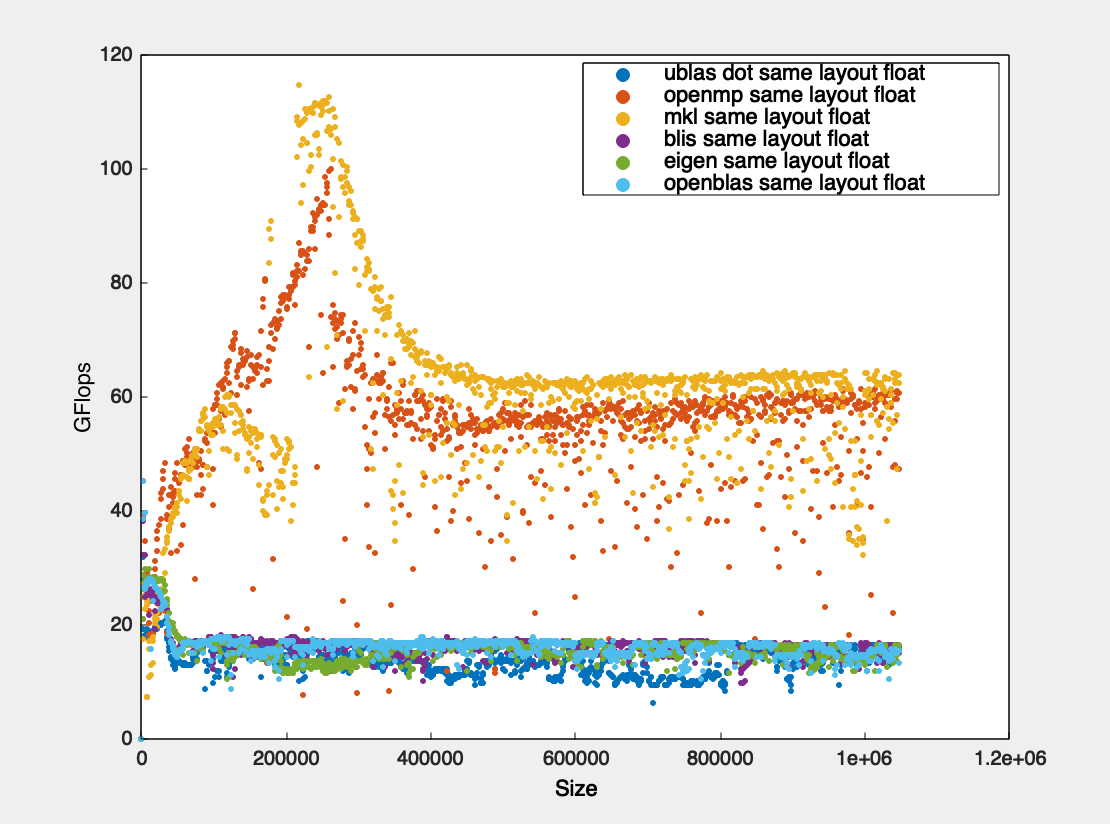
\includegraphics[width=8cm]{../assets/mtm/float_GflopsVsSize.png} }}%
    \label{fig:mtm_col_Sgflop220}
    \qquad
    \subfloat[\centering Double-Precision]{{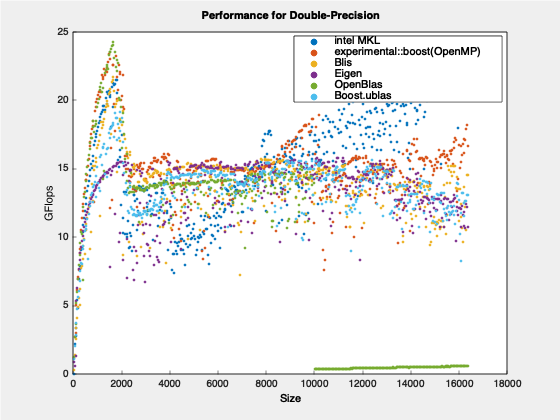
\includegraphics[width=8cm]{../assets/mtm/double_GflopsVsSize.png} }}%
    \label{fig:mtm_col_Dgflop220}
\end{figure}

\begin{figure}[htb]
    \centering
    \caption*{Sorted performance measurements of ?gemm implementations}
    \subfloat[\centering Single-Precision]{{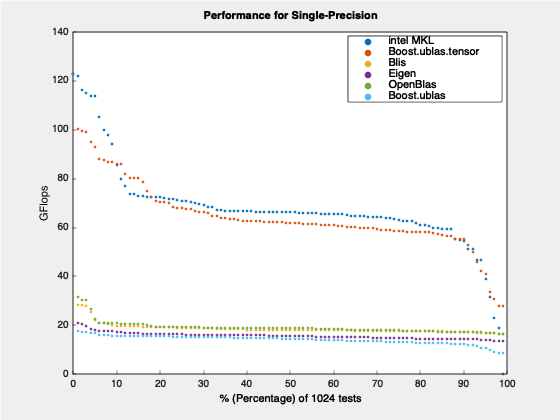
\includegraphics[width=8cm]{../assets/mtm/float_GflopsVsSize_per.png} }}%
    \label{fig:mtm_col_Sgflop_per220}
    \qquad
    \subfloat[\centering Double-Precision]{{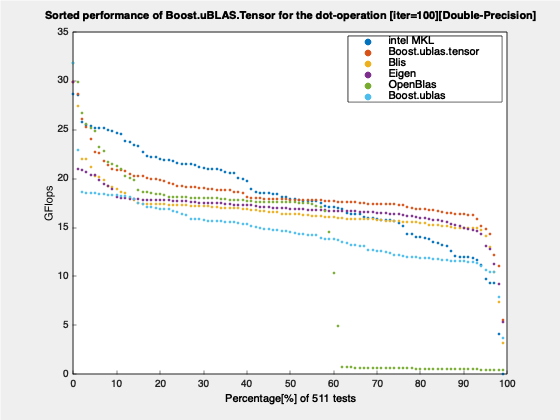
\includegraphics[width=8cm]{../assets/mtm/double_GflopsVsSize_per.png} }}%
    \label{fig:mtm_col_Dgflop_per220}
\end{figure}

\begin{figure}[htb]
    \centering
    \caption*{Comparison of the Boost.uBLAS.Tensor ?gemm implementation}
    \subfloat[\centering Single-Precision]{{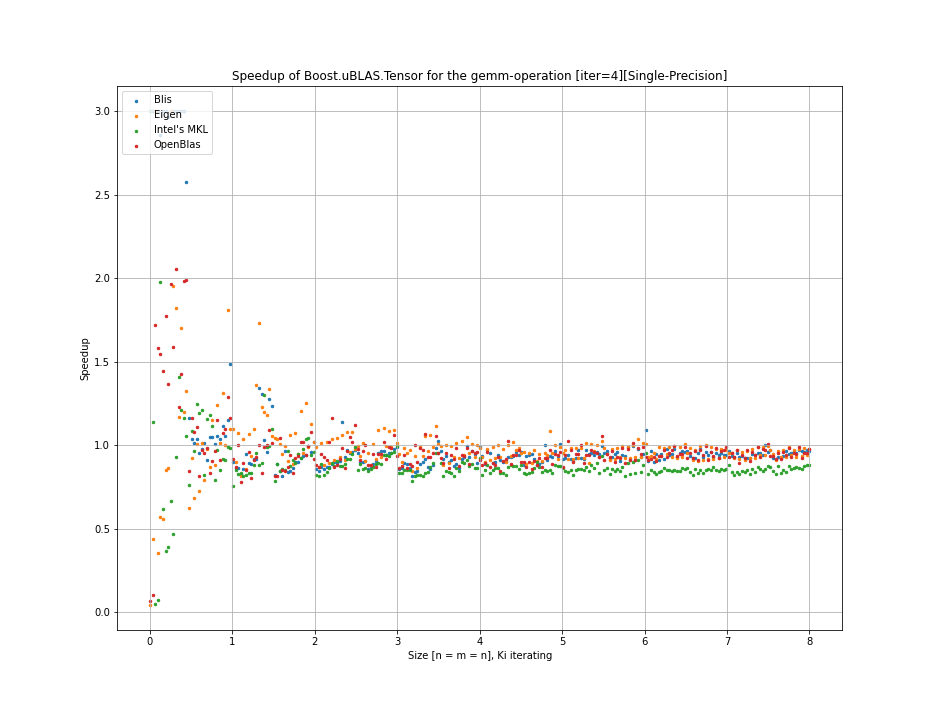
\includegraphics[width=8cm]{../assets/mtm/float_Speedup.png} }}%
    \label{fig:mtm_col_Sspeedup220}
    \qquad
    \subfloat[\centering Double-Precision]{{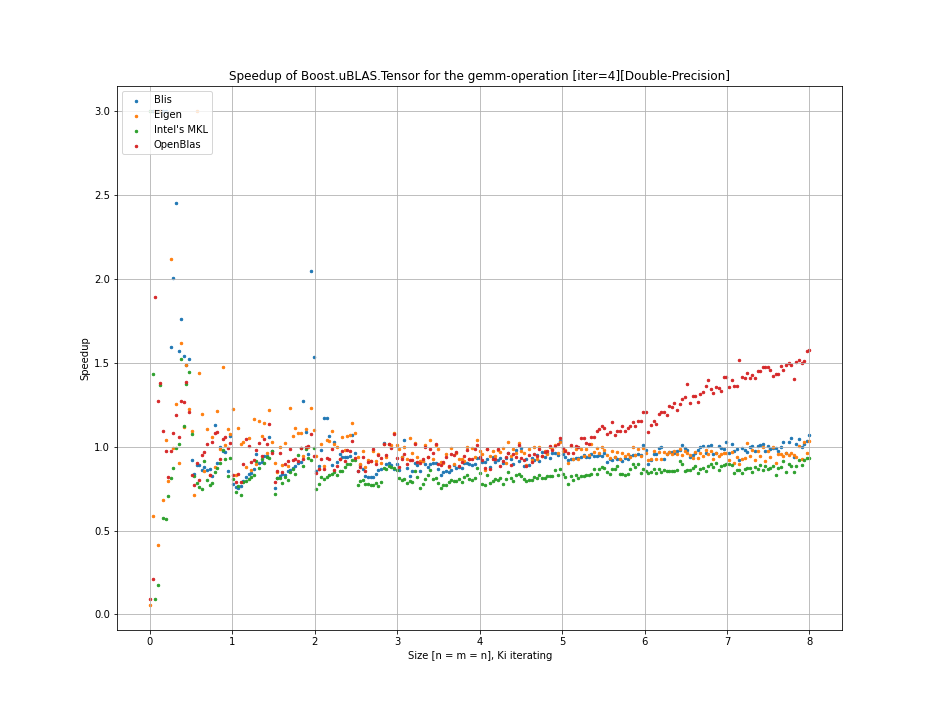
\includegraphics[width=8cm]{../assets/mtm/double_Speedup.png} }}%
    \label{fig:mtm_col_Dspeedup220}
\end{figure}

\begin{figure}[htb]
    \centering
    \caption*{Comparison of the Boost.uBLAS.Tensor ?gemm implementation [sorted]}
    \subfloat[\centering Single-Precision]{{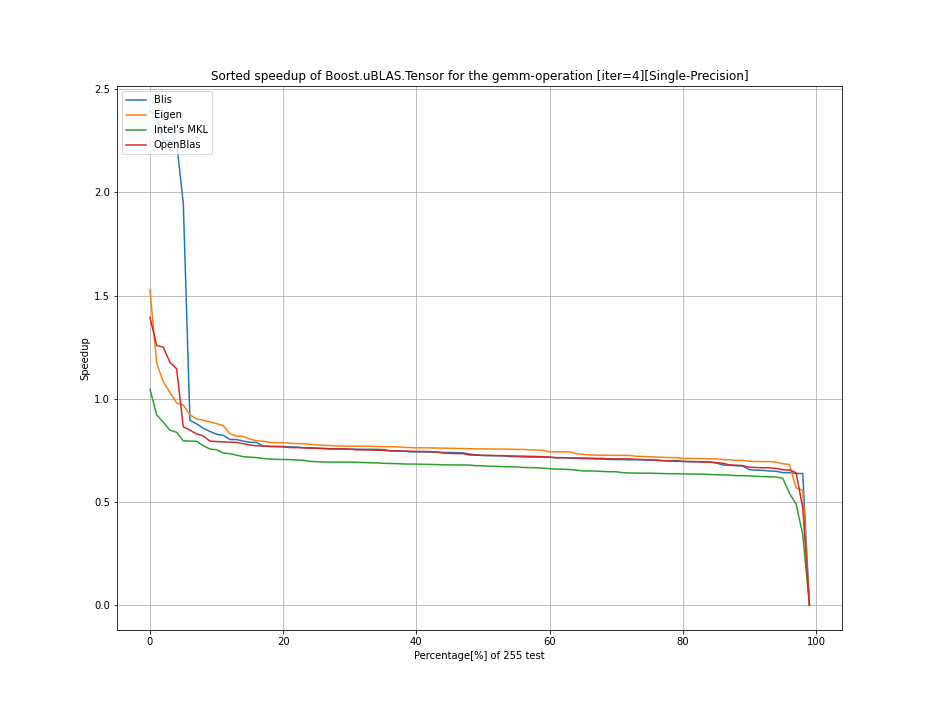
\includegraphics[width=8cm]{../assets/mtm/float_Speedup_per.png} }}%
    \label{fig:mtm_col_Sspeedup_per220}
    \qquad
    \subfloat[\centering Double-Precision]{{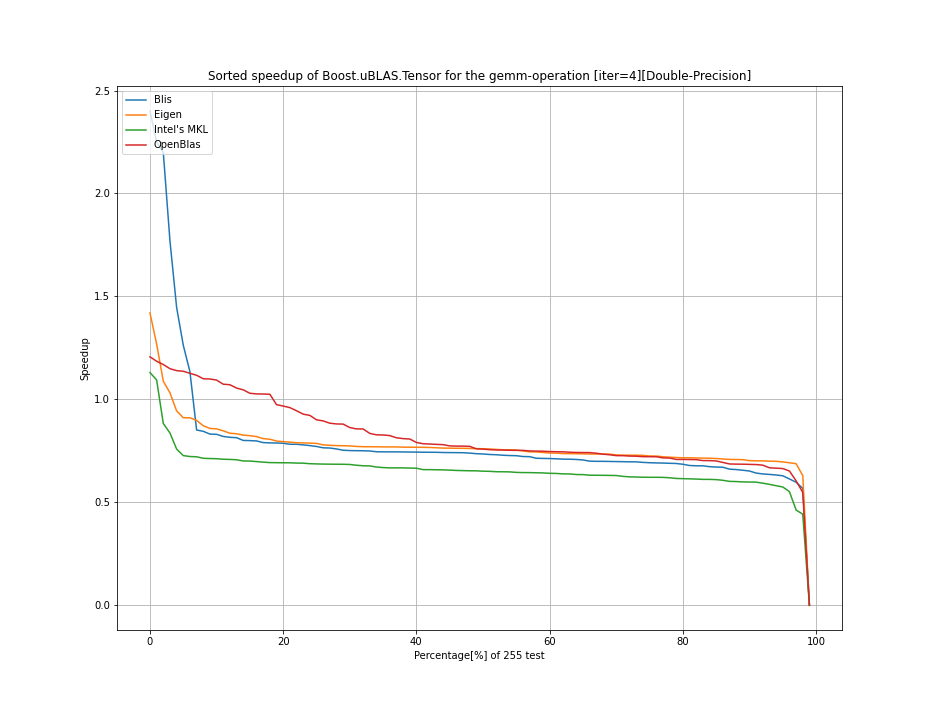
\includegraphics[width=8cm]{../assets/mtm/double_Speedup_per.png} }}%
    \label{fig:mtm_col_Dspeedup_per220}
\end{figure}

\begin{table}[ht]
    \centering
    \caption{Speedup Summary For Single-Precision}
    \begin{tabular}{|l|c|c|}
        \hline
        \textbf{Implementation} & \textbf{Speedup $\geq$ 1 [\%]} & \textbf{Speedup $\geq$ 2 [\%]}\\
        \hline
        OpenBLAS    & $4$ & $0$ \\
        \hline
        Eigen       & $3$ & $0$ \\
        \hline
        Blis        & $5$ & $4$ \\
        \hline
        Intel's MKL & $0$ & $0$ \\
        \hline
    \end{tabular}
    
    \begin{tabular}{|l|c|c|}
        \hline
        \textbf{Implementation} & \textbf{Speed-down $\geq$ 1 [\%]} & \textbf{Speed-down $\geq$ 2 [\%]}\\
        \hline
        OpenBLAS    & $99$ & $99$ \\
        \hline
        Eigen       & $99$ & $99$ \\
        \hline
        Blis        & $99$ & $99$ \\
        \hline
        Intel's MKL & $99$ & $99$ \\
        \hline
    \end{tabular}
    
    \vspace*{1 cm}

    \centering
    \caption{Speedup Summary For Double-Precision}
    \begin{tabular}{|l|c|c|}
        \hline
        \textbf{Implementation} & \textbf{Speedup $\geq$ 1 [\%]} & \textbf{Speedup $\geq$ 2 [\%]}\\
        \hline
        OpenBLAS    & $18$ & $0$ \\
        \hline
        Eigen       & $3$ & $0$ \\
        \hline
        Blis        & $6$ & $2$ \\
        \hline
        Intel's MKL & $1$ & $0$ \\
        \hline
    \end{tabular}
    
    \begin{tabular}{|l|c|c|}
        \hline
        \textbf{Implementation} & \textbf{Speed-down $\geq$ 1 [\%]} & \textbf{Speed-down $\geq$ 2 [\%]}\\
        \hline
        OpenBLAS    & $99$ & $99$ \\
        \hline
        Eigen       & $99$ & $99$ \\
        \hline
        Blis        & $99$ & $99$ \\
        \hline
        Intel's MKL & $99$ & $99$ \\
        \hline
    \end{tabular}
\end{table}

\clearpage
\subsection*{Range[Start: $32$, End: $8Ki$, Step: $32$]}

\begin{table}[ht]
    \centering
    \caption{GFLOPS For Single-Precision}
    \begin{tabular}{|l|c|c|}
        \hline
        \textbf{Implementation} & \textbf{Max} & \textbf{Average}\\
        \hline
        Boost.uBLAS.Tensor  & $698.297$& $577.354272$ \\
        \hline
        Intel's MKL         & $755.743$& $664.758359$ \\
        \hline
        OpenBLAS            & $739.551$& $607.188286$ \\
        \hline
        Blis                & $721.793$& $602.726757$ \\
        \hline
        Eigen               & $699.169$& $589.249039$ \\
        \hline
    \end{tabular}

    \vspace*{1 cm}

    \centering
    \caption{GFLOPS For Double-Precision}
    \begin{tabular}{|l|c|c|}
        \hline
        \textbf{Implementation} & \textbf{Max} & \textbf{Average}\\
        \hline
        Boost.uBLAS.Tensor  & $318.398$& $264.381474$ \\
        \hline
        Intel's MKL         & $368.052$& $312.992397$ \\
        \hline
        OpenBLAS            & $341.611$& $253.483622$ \\
        \hline
        Blis                & $342.725$& $278.499451$ \\
        \hline
        Eigen               & $320.632$& $268.866619$ \\
        \hline
    \end{tabular}
\end{table}

\begin{table}[ht]
    \centering
    \caption{Utilization[\%] For Single-Precision}
    \begin{tabular}{|l|c|c|}
        \hline
        \textbf{Implementation} & \textbf{Max} & \textbf{Average}\\
        \hline
        Boost.uBLAS.Tensor  & $118.596637$& $98.056092$ \\
        \hline
        Intel's MKL         & $128.353091$& $112.900537$ \\
        \hline
        OpenBLAS            & $125.603091$& $103.123011$ \\
        \hline
        Blis                & $122.587126$& $102.365278$ \\
        \hline
        Eigen               & $118.744735$& $100.076263$ \\
        \hline
    \end{tabular}

    \vspace*{1 cm}

    \centering
    \caption{Utilization[\%] For Double-Precision}
    \begin{tabular}{|l|c|c|}
        \hline
        \textbf{Implementation} & \textbf{Max} & \textbf{Average}\\
        \hline
        Boost.uBLAS.Tensor  & $108.151495$& $89.803490$ \\
        \hline
        Intel's MKL         & $125.017663$& $106.315352$ \\
        \hline
        OpenBLAS            & $116.036345$& $86.101774$ \\
        \hline
        Blis                & $116.414742$& $94.598998$ \\
        \hline
        Eigen               & $108.910326$& $91.326976$ \\
        \hline
    \end{tabular}
\end{table}

\begin{table}[ht]
    \centering
    \caption{Speedup(Boost.uBLAS.Tensor) For Single-Precision}
    \begin{tabular}{|l|c|c|}
        \hline
        \textbf{Implementation} & \textbf{Max} & \textbf{Average}\\
        \hline
        Intel's MKL         & $0.923987$& $0.868518$ \\
        \hline
        OpenBLAS            & $0.944218$& $0.950865$ \\
        \hline
        Blis                & $0.967448$& $0.957904$ \\
        \hline
        Eigen               & $0.998753$& $0.979814$ \\
        \hline
    \end{tabular}

    \vspace*{1 cm}

    \centering
    \caption{Speedup(Boost.uBLAS.Tensor) For Double-Precision}
    \begin{tabular}{|l|c|c|}
        \hline
        \textbf{Implementation} & \textbf{Max} & \textbf{Average}\\
        \hline
        Intel's MKL         & $0.865090$& $0.844690$ \\
        \hline
        OpenBLAS            & $0.932048$& $1.042992$ \\
        \hline
        Blis                & $0.929019$& $0.949307$ \\
        \hline
        Eigen               & $0.993033$& $0.983318$ \\
        \hline
    \end{tabular}
\end{table}
